\pdfinfoomitdate=1
\pdfsuppressptexinfo=15
\pdftrailerid{}
\documentclass[11pt,letterpaper]{article}
\usepackage[T1]{fontenc}
\usepackage{mathptmx}
\usepackage[scaled=.92]{helvet}
\usepackage[margin=.68in]{geometry}
\usepackage{microtype}
\usepackage{tikz}
\usetikzlibrary{arrows.meta,positioning,fit,calc}
\usepackage{booktabs,tabularx,array}
\usepackage{xcolor}
\usepackage[hidelinks,pdftitle={Bullet Farm Executive Brief},pdfauthor={Bullet Farm Maintainers},pdfsubject={Four-page executive architecture and assurance brief},pdfkeywords={Bullet Farm, software-change transaction, coding agents, evidence binding}]{hyperref}
% Generated from evidence.json by scripts/paper-build.sh. Do not edit.
\newcommand{\EvidenceSnapshotId}{20260825-stage1-r3}
\newcommand{\EvidenceSnapshotDate}{2026-08-25}
\newcommand{\EvidenceStage}{architecture-component-assurance}
\newcommand{\EvidenceHubCommit}{3039878371b6}
\newcommand{\EvidenceKernelCommit}{ca380bc4ffd4}
\newcommand{\EvidenceGitCommit}{fb715b25c3b2}
\newcommand{\EvidencePortalCommit}{95108e37d643}
\newcommand{\EvidenceDoctorOutcome}{BLOCKED}
\newcommand{\EvidenceReleaseOutcome}{BLOCKED}
\newcommand{\EvidenceReleaseEvaluated}{26}
\newcommand{\EvidenceReleaseBlocked}{26}
\newcommand{\EvidenceFastOutcome}{PASS}
\newcommand{\EvidenceDemoOutcome}{PASS}
\newcommand{\EvidenceFormalOutcome}{PASS}
\newcommand{\EvidenceFormalModels}{2}
\newcommand{\EvidenceAuditScore}{58}
\newcommand{\EvidenceAuditRaw}{58}
\newcommand{\EvidenceAuditCaps}{10}
\newcommand{\EvidenceAuditHard}{29}
\newcommand{\EvidenceAuditSoft}{15}
\newcommand{\EvidenceTransactionOutcome}{ABSENT}

% Shared vector figure used by the IEEE paper and executive brief.
\newcommand{\BulletArchitectureFigure}[1]{%
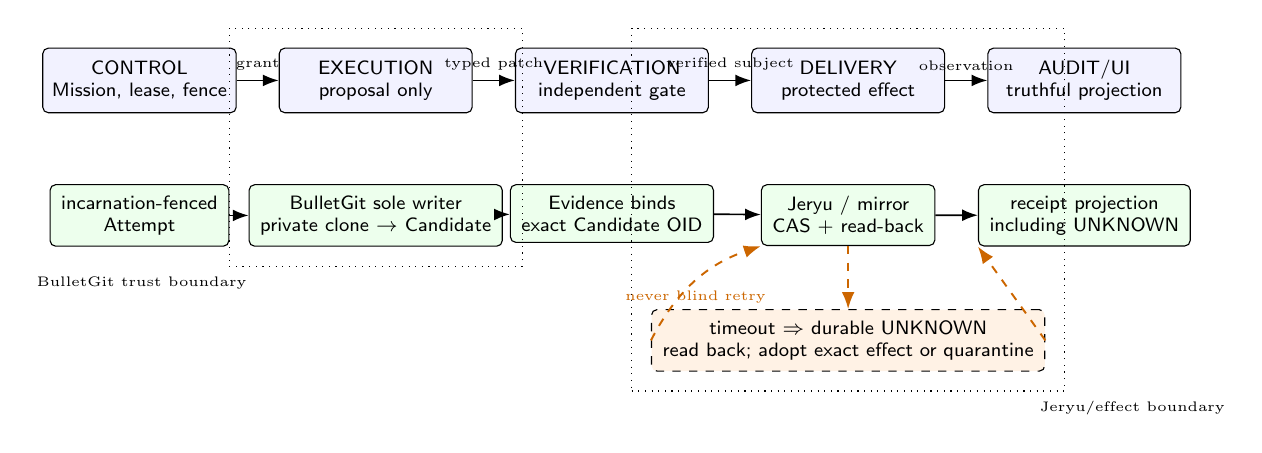
\begin{tikzpicture}[
  x=1cm,y=1cm,>=Latex,
  plane/.style={draw,rounded corners=2pt,minimum width=2.45cm,minimum height=.82cm,align=center,font=\sffamily\scriptsize,fill=blue!5},
  subject/.style={draw,rounded corners=2pt,align=center,font=\sffamily\scriptsize,fill=green!7,inner sep=4pt},
  warning/.style={draw,dashed,rounded corners=2pt,align=center,font=\sffamily\scriptsize,fill=orange!10,inner sep=4pt},
  flow/.style={->,line width=.6pt},
  reconcile/.style={->,dashed,line width=.7pt,color=orange!80!black}
]
\node[plane] (control) at (0,0) {CONTROL\\Mission, lease, fence};
\node[plane] (execution) at (3.0,0) {EXECUTION\\proposal only};
\node[plane] (verification) at (6.0,0) {VERIFICATION\\independent gate};
\node[plane] (delivery) at (9.0,0) {DELIVERY\\protected effect};
\node[plane] (audit) at (12.0,0) {AUDIT/UI\\truthful projection};

\node[subject,below=.9cm of control] (attempt) {incarnation-fenced\\Attempt};
\node[subject,below=.9cm of execution] (candidate) {BulletGit sole writer\\private clone $\rightarrow$ Candidate};
\node[subject,below=.9cm of verification] (evidence) {Evidence binds\\exact Candidate OID};
\node[subject,below=.9cm of delivery] (effect) {Jeryu / mirror\\CAS + read-back};
\node[subject,below=.9cm of audit] (projection) {receipt projection\\including UNKNOWN};

\draw[flow] (control) -- node[above,font=\tiny]{grant} (execution);
\draw[flow] (execution) -- node[above,font=\tiny]{typed patch} (verification);
\draw[flow] (verification) -- node[above,font=\tiny]{verified subject} (delivery);
\draw[flow] (delivery) -- node[above,font=\tiny]{observation} (audit);
\draw[flow] (attempt) -- (candidate);
\draw[flow] (candidate) -- (evidence);
\draw[flow] (evidence) -- (effect);
\draw[flow] (effect) -- (projection);

\node[warning,below=.8cm of effect] (unknown) {timeout $\Rightarrow$ durable UNKNOWN\\read back; adopt exact effect or quarantine};
\draw[reconcile] (effect) -- (unknown);
\draw[reconcile] (unknown.west) to[bend left=22] node[below,font=\tiny]{never blind retry} (effect.south west);
\draw[reconcile] (unknown.east) -- (projection.south west);

\node[draw,dotted,fit=(execution)(candidate),inner sep=7pt,label={[font=\tiny]below left:BulletGit trust boundary}] {};
\node[draw,dotted,fit=(delivery)(effect)(unknown),inner sep=7pt,label={[font=\tiny]below right:Jeryu/effect boundary}] {};
\end{tikzpicture}%
}

\pagestyle{plain}
\setlength{\parindent}{0pt}
\setlength{\parskip}{4pt}
\setlength{\emergencystretch}{2em}
\newcommand{\statusbox}[1]{\colorbox{blue!8}{\parbox{.96\linewidth}{#1}}}
\newenvironment{tight}{\setlength{\topsep}{1pt}\setlength{\partopsep}{0pt}\begin{itemize}\setlength{\itemsep}{1pt}\setlength{\parskip}{0pt}\setlength{\parsep}{0pt}}{\end{itemize}}
\newcommand{\block}[2]{\vspace{1pt}\textbf{#1}{\footnotesize\ #2}\par\vspace{-2pt}}
\newenvironment{tightenum}{\setlength{\topsep}{1pt}\setlength{\partopsep}{0pt}\begin{enumerate}\setlength{\itemsep}{1pt}\setlength{\parskip}{0pt}\setlength{\parsep}{0pt}}{\end{enumerate}}

\begin{document}
\begin{center}
{\LARGE\bfseries Bullet Farm}\par
\vspace{1pt}
{\Large A transaction processor around powerful coding agents}\par
\vspace{2pt}
{\small Executive brief --- Stage-1 architecture and component assurance --- 25 August 2026}
\end{center}

{\large\bfseries Decision summary}\par
\small\setlength{\parskip}{3pt}
\block{What it is.}{}
\begin{tight}
\item A software-change transaction processor \emph{around} coding agents
(Claude, Codex, Cursor, Antigravity, others). Agents reason and propose
patches; they never hold repository, verification, or merge authority.
\item Four repositories (Hub, Kernel, BulletGit, Portal) across five trust
planes (control, execution, verification, delivery, audit), so no plane can
use its own assertion as evidence.
\end{tight}

\block{What it is worth if it works.}{}
\begin{tight}
\item \emph{Teams running many agents} stop losing work to seven recurring
failures: two writers on one checkout, a stale process that still writes,
tests that name a moved branch, a timed-out push retried into a duplicate,
silence read as death or success, cleanup before preservation, and a dashboard
that paints missing state green (Gas Town \#4094/\#3584/\#4737/\#4091, Gas
City \#1181/\#5511/\#1052 are public instances).
\item \emph{Reviewers and auditors} get, for every integrated change, exact
evidence of who observed which bytes under which admitted gate; a rebase,
gate, or policy change invalidates it instead of carrying stale green.
\item \emph{Operators} swap models and vendors without changing who may write;
cost, refusal, and unresolved unknowns are recorded per change. The target
metric, accepted surviving change per human intervention and per dollar, is a
Stage-2 measurement, not a claim here.
\item \emph{Later:} bounded multi-agent evolution over evidence lineages (Designed; post-V1).
\end{tight}

\block{What is proven today.}{Snapshot \EvidenceSnapshotId: Hub
\EvidenceHubCommit, Kernel \EvidenceKernelCommit, BulletGit
\EvidenceGitCommit, Portal \EvidencePortalCommit.}
\begin{tight}
\item Component-proved only: fast \EvidenceFastOutcome, demo
\EvidenceDemoOutcome, contract, registry, and required lanes PASS,
\EvidenceFormalModels{} bounded TLA+ safety models \EvidenceFormalOutcome.
\item Not proved: \texttt{TRANSACTION\_PROOF} \EvidenceTransactionOutcome;
live provider, forge, and release proof absent; doctor
\EvidenceDoctorOutcome{} by design; \EvidenceReleaseBlocked{} blocked of
\EvidenceReleaseEvaluated{} release gates (\texttt{check release}, exit 3).
\item Security audit \EvidenceAuditScore{} (raw \EvidenceAuditRaw),
\EvidenceAuditCaps{} caps, \EvidenceAuditHard{} hard findings; release floor 90/0/0.
\end{tight}

\block{Biggest concerns.}{Ranked; the paper names the receipt that retires each.}
\begin{tight}
\item Connected product unassembled: 0 of 26 gates receipted; every positive
result is component-level; the family's own weighted self-assessment is
26/100 (a planning judgment, not a receipt).
\item No live evidence at this subject: the committed policy refuses every
provider before spawn; no authenticated Jeryu or GitHub read-back exists.
\item Closure needs operator custody acts: live-admission ratification, Jeryu
authentication, release signing keys, schema-3 lock inputs.
\item Single host, Linux only, same UID; some Git/helper paths remain raceable; macOS/Windows refuse.
\item Verifier independence rests on one fixture gate and human-curated
holdouts; a later evolutionary layer inherits that dependence.
\item Security score below its own floor; no portable hosted audit artifact.
\item Split-brain, quota, and liveness are bounded, not eliminated; formal models are bounded safety only.
\item Size, cost, adoption: five planes, 26 gates, private-clone storage,
read-back latency; only Jeryu and a GitHub adapter specified; cost unmeasured.
\end{tight}

\block{What must happen before launch.}{Predecessor order; owner in parentheses.}
\begin{tight}
\item Operator ratifies live admission (policy generation 2, provider-runner
key) and supplies Jeryu authentication, signing custody, schema-3 lock inputs
(operator: G1, G5, G6, G7).
\item One signed connected five-plane \texttt{TRANSACTION\_PROOF} (engineering:
G2--G4), then sealed live receipts for four providers and Jeryu/GitHub
read-back (both: G5--G7).
\item Audit at floor with a portable CI artifact; five signed packages with
SBOM, provenance, checksums; installer twice in a fresh home; platform
refusal receipts (engineering: G8--G10).
\item Only then the Stage-2 matched benchmark, before any ``faster, cheaper,
safer'' claim.
\end{tight}
\normalsize

\newpage
\section*{Why this is powerful: the binding chain}

Four questions decide whether agent work survives: \emph{who owns the write,
which incarnation is current, which exact bytes were proved, and did the remote
mutation really happen?} A sandbox, worktree, reviewer, or merge queue answers
at most one, which is why an agent can reason brilliantly and still lose work
when two sessions share a checkout, a retry duplicates a workflow, CI approves
a branch that moved, or a dashboard reads silence as success. Bullet Farm puts
all four answers outside the model; providers propose, and the repository
remains sovereign even when models and vendors are swapped.

\begin{center}
\resizebox{.8\textwidth}{!}{\BulletArchitectureFigure{\textwidth}}
\end{center}

The design composes eight bindings: incarnation fence $\rightarrow$ sole
writer $\rightarrow$ private Attempt clone $\rightarrow$ exact-OID Candidate
$\rightarrow$ independent Evidence $\rightarrow$ durable effect intent
$\rightarrow$ read-back/adoption $\rightarrow$ truthful projection.

\begin{tightenum}
\item \textbf{Concurrency becomes explicit.} A lease plus an incarnation fence
means a process that wakes after reclaim is stale, even if it still runs.
\item \textbf{Git identity becomes exact.} One BulletGit writer applies typed
patches in private Attempt clones and mints an immutable Candidate from exact
base, head, tree, and provenance subjects.
\item \textbf{Evidence cannot float.} An independent verifier proves that
Candidate, not a moving branch, a transcript, or a model's ``done'' statement.
\item \textbf{Timeout is survivable.} Durable effect intent plus read-back
distinguishes applied, not applied, and honest \texttt{UNKNOWN}; an ambiguous
push is never blindly retried.
\item \textbf{The UI cannot manufacture truth.} Projections retain stale,
contradictory, failed, and unknown outcomes instead of painting them green.
\end{tightenum}

\section*{A failure, recovered without guessing}

Suppose a protected-ref update times out after the forge may have accepted it.
A conventional retry loop assumes failure and sends the mutation again. Bullet
Farm has already committed one logical effect identity, expected-old OID,
intended-new OID, and Evidence root; it records \texttt{UNKNOWN} and reads back:

\begin{tabularx}{\textwidth}{@{}p{.19\textwidth}X@{}}
\toprule
Observed state & Required action \\
\midrule
Ref equals intended OID & Adopt the already-applied effect and seal the read-back receipt. \\
Ref equals expected-old OID & Retry the same logical effect identity under the current fence. \\
Ref equals neither & Quarantine divergence; preserve bytes and require adjudication. \\
No trustworthy observation & Remain \texttt{UNKNOWN}; do not infer success or failure. \\
\bottomrule
\end{tabularx}

The unit that matters is not a chat session but this recoverable journey from
authority to exact Candidate, Evidence, protected effect, and observation.

\newpage
\section*{Implemented now / not yet proved}

\statusbox{\textbf{Prominent limit.} Every positive Bullet result below is
component evidence. \texttt{TRANSACTION\_PROOF}, live-provider/forge proof,
and release proof are absent. The release inventory is
\EvidenceReleaseOutcome: \EvidenceReleaseBlocked{} blocked of
\EvidenceReleaseEvaluated{} evaluated gates.}

\small
\renewcommand{\arraystretch}{1.14}
\begin{tabularx}{\textwidth}{@{}p{.20\textwidth}X X@{}}
\toprule
Boundary & Implemented now & Not yet proved \\
\midrule
Control authority & DB-clock lease/fence, atomic command/outbox, quarantined signed lease-transport & Connected reservation/settlement from Kernel through Runner and BulletGit \\
Provider boundary & Offline protocol subsets, admission and egress components, policy-first refusal & Any live provider receipt; live policy remains disabled in the evidence subject \\
Repository writer & Fail-closed BulletGit gateway, private-clone/preservation components, strict manifests & Positive online sole-writer path; public clone still refuses as \texttt{AUTHORITY\_CONTRACT\_UNAVAILABLE} \\
Candidate/Evidence & Exact-subject fixture gate and bounded verifier transport & Production reconstruction, executable identity for all gates, multi-gate aggregation \\
Effects & Ambiguity model and local bare-forge components & Authenticated expected-old-OID push, read-back, adoption, and protected integration \\
Audit/Portal & Generated DTOs, exact command reconciliation, watermark projections, explicit \texttt{UNKNOWN} & Packaged complete product and every designed ledger subject \\
Formal assurance & \EvidenceFormalModels{} bounded safety models, \EvidenceFormalOutcome{} at pinned state counts & Liveness, OS/Git/provider/forge composition, or a product proof \\
Release & Negative inventory; audit \EvidenceAuditScore{}/raw \EvidenceAuditRaw, \EvidenceAuditCaps{} caps, \EvidenceAuditHard{} hard findings & Quality floor, portable audit, packages, SBOM/provenance, signing, install/recovery, live receipts \\
\bottomrule
\end{tabularx}
\normalsize

\section*{How to read maturity}

\begin{tabularx}{\textwidth}{@{}p{.23\textwidth}X@{}}
\textsf{Designed} & Reviewed rule; executable path may not exist. \\
\textsf{Component-proved} & Exact committed component plus mapped receipt; no cross-plane inference. \\
\textsf{Transaction-proved} & One exact connected offline five-plane transaction with independent receipts. \\
\textsf{Live/release-proved} & Admitted live provider/forge transaction, or signed package/install/recovery proof. \\
\end{tabularx}

The snapshot reports doctor \EvidenceDoctorOutcome, fast
\EvidenceFastOutcome, demo \EvidenceDemoOutcome, and transaction proof
\EvidenceTransactionOutcome. Demo success is not silently relabeled as a
transaction. A timeout, skip, unsupported path, missing receipt, or dirty-tree
result cannot be promoted through prose.

\section*{The practical consequence}

Bullet Farm is powerful as a control architecture now, but not yet proved as a
connected product. That distinction is a feature: it makes investment and risk
decisions against a visible boundary instead of a polished demonstration.

\newpage
\section*{What adjacent systems contribute}

Gas Town and Gas City provide strong orchestration, durable work, multiple
runtimes, and merge-queue operations; DeepSeek Harness a composable plugin
kernel plus an experimental Teams seam; Omnigent cross-vendor sessions,
parallel worktrees and review, OS sandboxes, and an L7 credential proxy.
Bullet Farm should retain those lessons. Its narrower claim is that the
reviewed pinned public contracts do not document this same end-to-end
authority/evidence/effect chain; linked worktrees, for example, share the
object database and most refs and are not separate repository principals.

\section*{Publication, forge topology, and next decisions}

\subsection*{Two publication stages}

\textbf{Stage 1 --- now.} Publish the architecture and component-assurance
preprint, the four-page brief, bibliography, vector figure, JSON evidence
snapshot, generated macros, and deterministic preflight. Make no comparative
performance claim.

\textbf{Stage 2 --- later.} Only after a signed connected
\texttt{TRANSACTION\_PROOF}, run a matched receipt-bearing corpus against pinned
systems, recording tasks, subjects, models, budgets, retries, costs,
collisions, duplicate effects, unknowns, recovery, and loss. Only this stage
may support ``faster,'' ``cheaper,'' ``safer,'' or ``more successful.''

\subsection*{Frozen V1 topology and blocked proposals}

\begin{itemize}
\item V1 source distribution is Jeryu-only from immutable signed tags. The
manifest admits no authenticated Jeryu URL and assumes no public mirror.
\item The only permitted local Jeryu family is
\texttt{/home/ubuntu/jain-split/jeryu-split}; its branded hub maps independent
component repositories. Never recreate \texttt{/home/ubuntu/jeryu-split}.
\item \texttt{git.neverhuman.org}, \texttt{github.com/neverhuman/jeryu}, and
\texttt{github.com/neverhuman/jankurai} are unratified, operator-blocked future
proposals. GitHub may later be chosen as a public index or backup, and
independent Jeryu Git as a hosted front door; neither is authority today.
\item Any later public mirror remains a separately configured effect adapter.
It requires expected-old-OID CAS, read-back, divergence quarantine, and
separately proved backups.
\item Jankurai stays the existing monorepo at \texttt{/home/ubuntu/jankurai}.
No public front door is assumed; preservation must precede any mirror decision.
\item The local-family rule is frozen; the endpoint and mirror proposals are
not. Operator ratification plus TLS, auth, protection, deployment, mirror,
backup, and restoration receipts precede any name becoming authority.
\end{itemize}

\subsection*{Immediate decisions}

\begin{tightenum}
\item Fund the connected five-plane transaction proof before comparative marketing.
\item Publish immutable signed \texttt{bullet-wire} only through an operator-ratified, authenticated Jeryu endpoint.
\item Select and prove protected Jeryu integration plus the ratified endpoint's operational controls.
\item Finish deterministic packages, SBOM/provenance, schema-3 installation, and portable Jankurai audit evidence.
\item Resolve Jeryu release-authority document drift and preserve Jankurai history before any mirror decision.
\item Publish immutable paper/source permalinks only after strict preflight is green from clean subjects.
\end{tightenum}

\vfill
\statusbox{\textbf{Bottom line.} More capable models increase the value of
external authority, exact evidence, and recoverable effects. Bullet Farm has a
defensible transaction architecture and meaningful components. It does not yet
have the connected proof needed to claim a finished product or measured
superiority.}

\end{document}
